\documentclass[../main.tex]{subfiles}
\graphicspath{{\subfix{../../Images}}}

\begin{document}
\section{Results and Comparison}
\label{sec:results_and_comparison}

\subsection{Technology Comparison}
The implementation exercise depicted in Sec. \ref{sec:solidity_ethereum_nft_implementation} and Sec. \ref{sec:cadence_flow_nft_implementation} provided sufficient data to do a side-by-side comparison between the two blockchains technologies considered.
\par
Table \ref{tab:ethereum_flow_comparison_table} summarises the technological characteristics that set these blockchain technologies apart.


% Please add the following required packages to your document preamble:
\begin{table*}[h]
    \footnotesize
    \caption{Architectural comparison between Ethereum and Flow blockchains}
    \centering
    \begin{adjustwidth}{-1.5cm}{}
        \begin{tabular}{@{} m{4cm} ll@{}}
            \toprule
            \multicolumn{1}{c}{\multirow{2}{*}{\textbf{Parameter}}} & \multicolumn{2}{c}{\textbf{Non-Fungible Architecture}}                                                     \\ \cmidrule(l){2-3}
            \multicolumn{1}{c}{}                                    & \multicolumn{1}{l}{\textbf{Ethereum}}                               & \textbf{Flow}                        \\ \midrule
            \textbf{Year}                                           & \multicolumn{1}{l}{2013}                                            & 2020                                 \\ \midrule
            \textbf{Native Cryptocurrency}                          & \multicolumn{1}{l}{ETH}                                             & FLOW                                 \\ \midrule
            \textbf{Virtual Machine}                                & \multicolumn{1}{l}{EVM (Ethereum Virtual Machine)}                  & FVM (Flow Virtual Machine)           \\ \midrule
            \parbox[m]{4cm}{\textbf{Smart Contract                                                                                                                               \\Programming Language}} & \multicolumn{1}{l}{Solidity}                                        & Cadence                              \\ \midrule
            \textbf{Consensus Algorithm}                            & \multicolumn{1}{l}{2013-2022: Proof-of-Work, 2022-: Proof-of-Stake} & Proof-of-Stake                       \\ \midrule
            \multirow{4}{*}{\textbf{Network Nodes Role Type}}       & \multicolumn{1}{l}{\multirow{2}{*}{1 - Execution Client}}           & 1 - Collector Node                   \\ \cmidrule(l){3-3}
                                                                    & \multicolumn{1}{l}{}                                                & 2 - Consensus Node                   \\ \cmidrule(l){2-3}
                                                                    & \multicolumn{1}{l}{\multirow{2}{*}{2 - Consensus Client}}           & 3 - Execution Node                   \\ \cmidrule(l){3-3}
                                                                    & \multicolumn{1}{l}{}                                                & 4 - Verification Node                \\ \midrule
            \multirow{2}{*}{\textbf{Token Standards}}               & \multicolumn{1}{l}{ERC-20 (fungible token standard)}                & FungibleToken                        \\ \cmidrule(l){2-3}
                                                                    & \multicolumn{1}{l}{ERC-721 (non-fungible token standard)}           & NonFungibleToken                     \\ \midrule
            \textbf{Data Storage Architecture}                      & \multicolumn{1}{l}{Contract-based}                                  & Account(User)-based                  \\ \midrule
            \textbf{Block Rate (Average)}                           & \multicolumn{1}{l}{12 - 15 seconds per block}                       & 0.5 - 1 seconds per block            \\ \midrule
            \textbf{Volume of daily transactions submitted (2024)}  & \multicolumn{1}{l}{1 - 1.25 million transactions per day}           & 0.5 - 1 million transactions per day \\ \midrule
            \textbf{Average gas price per transactions}             & \multicolumn{1}{l}{5.5 gwei ($\sim$0.39 \$)}                        & $\sim$0.00000845 \$                  \\ \bottomrule
        \end{tabular}
    \end{adjustwidth}
    \label{tab:ethereum_flow_comparison_table}
\end{table*}


\subsubsection{Analysis}
As it was mentioned in Sec. \ref{sec:flow_background}, Flow was created as a response to the limitations exposed by the earlier Non-Fungible Token projects. Ethereum had its official origin at the end of 2013, with the publication of Ethereum's first white paper \cite{Buterin2014}, the first Ethereum NFT projects introduced in 2015 and, by the end of 2017, the \textit{CryptoKitties} project had evidenced the limitations of this blockchain regarding its capacity to deal with spikes in NFT activity in the network. The team behind the \textit{CryptoKitties} project took the 3 years that followed to develop a new blockchain concept to solve those and published their solution in 2020 as Flow, a new blockchain into the ecosystem. During this period, Ethereum begun by using the \textit{Proof-of-Work} consensus algorithm but this chain was forked in September 2022 (the Paris fork which implemented \textit{EIP-3675} \cite{EIP3675}) and the mainnet consensus protocol was switched to a more energy friendly and efficient \textit{Proof-of-Stake}. The advantages of PoS vs. PoW were well identified by 2020, so Flow was created with a PoS consensus protocol from the beginning.
\par
Both blockchains run computations through a similar virtual machine abstraction, both named suggestively, but based in different, but comparable, node architectures. Ethereum establishes its \textit{Ethereum Virtual Machine} through a 2 node architecture that split all EVM operations into either \textit{executions} or \textit{consensus} operations, with the nodes in this network being split between these two roles. Flow identifies this architectural aspect as a limiting one regarding the scalability of the network and suggested a 4-node architecture with explicit purpose of pipelining computations in their \textit{Flow Virtual Machine} and to establish a \textit{Resource}-based computational paradigm, as it was detailed previously in Sec. \ref{sec:cadence_resource_oriented_paradigm}. This factor is evident in the average block rates for each case. Flow displays a block rate between 12 to 30 times faster than Ethereum, which results in faster transaction confirmations and computations besides having a more complex node architecture, thus supporting the claims for higher scalability from Flow.
\par
Another architectural feature that distinguish these technologies is the storage model used to save data in the blockchain. Ethereum uses a contract-based model, where all ownership relations are implemented as key-value mappings stored in the smart contract itself, while Flow uses a account-based storage model where each user account also controls an individual storage space associated to that account and all digital objects owned by this account are saved in this space and nowhere else. Ethereum's model is simpler and easier to implement, but creates access bottlenecks by funneling all project-related transactions to go through the main smart contract, as well as establishing a ownership weak spot in the contract itself as well. All NFT ownership records are saved in the Ethereum smart contract, therefore if this contract becomes unavailable, so do all NFT records. Flow solves this limitation by establishing resource types that can exist "outside" of the implementing contract, while allowing these resources to be independently saved in a account storage space. This decoupling makes a NFT independent of its issuing contract, i.e., a NFT in Flow can exist in the ecosystem even if the original contract does not. It also removes the access bottleneck from before. The issuing Flow contract is usually accessed only to mint a NFT. Once this resource is created, it typically moved to the owner's storage space and from there can be moved to another user accounts using a standardised transfer functions that are inherited from the token standards. As long as these standard are deployed and available in the network, tokens can be manipulated even if the issuing contracts no longer exist. Ethereum provides a similar functionality regarding standard functions such as transfer, balanceOf, ownerOf, etc., but because the ownership mappings are always stored in the implementing contract, if this element is destroyed, the whole ownership chain is destroyed as well. Flow prevents this by decentralising its storage architecture into an account-based system.
\par
Comparing both blockchains regarding their daily transaction average or the average gas price is merely illustrative because these values include a significant factor of popularity that does not translate directly into objective characteristics passible to be compared. Ethereum has a much slower block rate and very expensive gas prices when compared to Flow, but it still displays a daily transaction average that is the same as Flow in its lower end, but can be as much as 2.5 times larger. This is mainly due to popularity, which also drives price speculations, which justifies the large difference between average gas prices (An Ethereum transaction costs, in average, more expensive by a factor of 46154) as well as the increased daily transaction averages. Ethereum is 7 years ahead of Flow and it as also being used as the default blockchain for smart contract based projects, since it was the first public blockchain to offer explicit support for it. The elements that drive this price difference fall outside the bounds of this study, but it is important to node the massive difference that these may cause in blockchain usability.
\par
Both blockchains define strict standards to regulate token mechanics in their chains, both of the fungible and non-fungible type. This creates a normalised application space where projects created by different development teams can interact with each other without any pre-arrange conventions, as long as both have the care to implement their tokens through the official standards. In both cases, these standards are abstracted into contract interfaces, that at their core are files that explicit mandatory structures and functions for any token implemented. The standards indicated in Table \ref{tab:ethereum_flow_comparison_table} were discussed previously in greater detail in Sec. \ref{sec:token_standards}.


\subsection{Cost Analysis}
\label{sec:cost_analysis}
Another important aspect from smart contract supporting blockchains is characterising how these manage the delegation of distributed computations, which is typically regulated with a cost structure based on charging \textit{gas} to encourage users to deploy optimised code and to prevent abuses from malicious/erroneous code. Both Ethereum and Flow implement a \textit{gas} fee structure used to pay for transaction costs. At a fundamental level the two systems are very similar, namely, the blockchain charges small fractions of a native cryptocurrency token to pay for computational costs.
\par
For this study, the contracts indicated in Sec. \ref{sec:solidity_ethereum_nft_implementation} and Sec. \ref{sec:cadence_flow_nft_implementation} were deployed in an emulator environment. The \textit{Hardhat} Solidity development framework was used to analyse the Ethereum contract, namely, using its internal EVM emulator, while Flow streamlines this aspect of development, providing a built-in emulator environment with the command line interface, which was used for this purpose as well.
\par
For each case, a service/emulator account was used for contract deployment and other admin-level operations, such as minting a new NFT, while other, general-purpose accounts were used to emulate independent accounts that could receive, transfer, and burn NFTs. Each blockchain was analysed cost wise for a set of the most common operations while dealing with an NFT-based project, namely:
\begin{enumerate}
    \item {Deploy the NFT contract}
    \item {Mint a new NFT into a user account}
    \item {Transfer the NFT between user accounts}
    \item {Burn the NFT}
\end{enumerate}

\subsubsection{Ethereum Fee System}
Ethereum defines its gas in \textit{gwei}, a denomination of ETH, where 1 \textit{gwei} $ = 1 \times 10^{-9} $ ETH. The total transaction fee is split into two fee components: a \textit{base} fee and a \textit{priority} fee. The base fee is defined at the protocol level and is proportional to the computations that are required by the transaction. The priority component is added to the base one to make the transaction more attractive to validator and thus increase its probability of being included in the next block \cite{ethereum2024c}. The total amount to pay is calculated with:
$$
    total\: transaction\: fee = unit\: of\: gas\: used \times ( base\: fee + priority\: fee)
$$

The Hardhat development framework used in this exercise provides a built-in \textit{gas reporter} tool that provides a concise summary of the gas consumed by a sequence of operations defined in a script. The operations indicated in Sec. \ref{sec:cost_analysis} were included in an script and Table \ref{fig:solidity_gas_cost} displays the results returned from the gas reporter tool:

% // TODO: Replace this table by a latex one
\begin{figure}[htp]
    \centering
    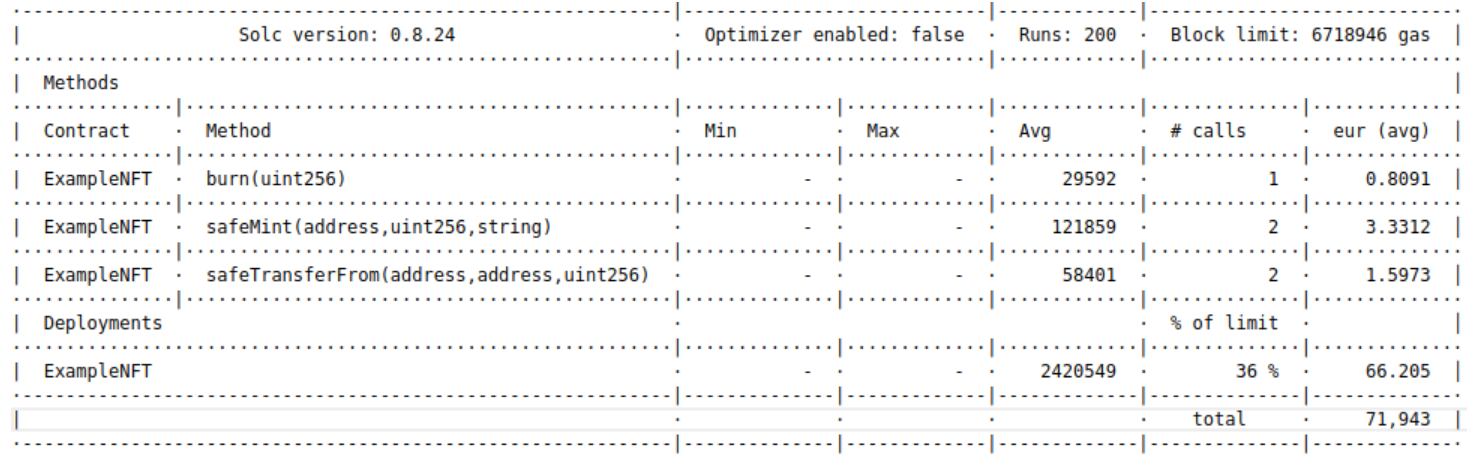
\includegraphics[width=1.0\textwidth]{../Images/11_solidity_fee_calculation.png}
    \caption{Gas consumption report from Hardat's gas reported tool}
    \label{fig:solidity_gas_cost}
\end{figure}

The report returned provided a global overview of how much each transaction costs but does not indicates which account paid the costs. The deployment of the contract and minting of NFT were paid by the service account while the remaining operations were paid by the account that owned the NFT. Overall, Ethereum is a notoriously expensive blockchain to operate. The ETH token is often subject of speculative periods which elevate its price above how useful the token really is. One one end, Ethereum provides a more standardised environment, given that most academic research on blockchain technology has largely preferred this blockchain. But from a practical implementation point of view, the current price to pay for basic NFT operability is prohibitive.

\subsubsection{Flow Fee System}
Flow implements a similar system to Ethereum to regulate distributed computations in the virtual machine. Flow does not define a gas unit per se, given that FLOW does not establishes any sub units for the moment, but it does define a minimum transaction fee of 0.000001 FLOW, unlike Ethereum. FLOW tokens are significantly cheaper than ETH (< 1 € per FLOW vs > 3000 € per ETH in 2024), so it makes sense to establish a minimum value for this blockchain. Flow transactions fees are also component based. The total transaction cost depends from three fee components:
\begin {itemize}
\item {An Inclusion fee} to pay for the inclusion of the transaction into a block, transporting information within the network and validating transaction signatures. Currently this value is fixed to the minimum transaction value of 0.000001 FLOW.
\item {An Execution fee} to pay for FVM computations, namely, interpreting lines of code, reading and writing in storage, creating accounts, etc.
\item {A Surge factor} applied dynamically depending on network usage. This factor is yet to be implemented in the protocol but it is intended to be used to modulate network usage spikes: when the network is too busy, this factor increases to encourage users to delay transactions, while a low factor during network idle times can be use to encourage user activity.
\end{itemize}

The total costs for a Flow transaction can be calculated with:
$$
    total\: transaction\: cost = (execution\: fee + inclusion\: fee) \times surge\: factor
$$

Unfortunately, Flow command line interface does not provides a gas reporter or similar tool, but interacting with this blockchain is significantly more verbose than with Ethereum. Also, Flow implements a standard for fee processing, namely the FlowFees contract. This contract is deployed in mainnet, testnet and by default in an emulator instance. Gas fees are paid directly to this contract and every time a successful fee payment is registered, the contract emits a specific event, namely \textit{FlowFees.FeesDeducted}, with the total fee paid, the inclusion fee and the execution fee as arguments. Though not ideal, it does provide a easy method to determine fee costs.
\par
Alternatively, it is relatively easy to query the Flow blockchain to obtain FLOW balances and even the current storage level, which relates to the total costs by the storage scheme used by Flow that was described in Sec. \ref{sec:storage_in_flow}, for each account involved. As such, the cost exercise was repeated for the Flow blockchain. Table \ref{fig:cadence_gas_cost} presents a study on how the main balance and internal storage levels fluctuate during the lifecycle of a NFT in Flow

% // TODO: Replace this table by a latex one
% // TODO: Split this table into gas and space analysis, add the rest of the accounts and redo the analysis
\begin{figure}[htp]
    \centering
    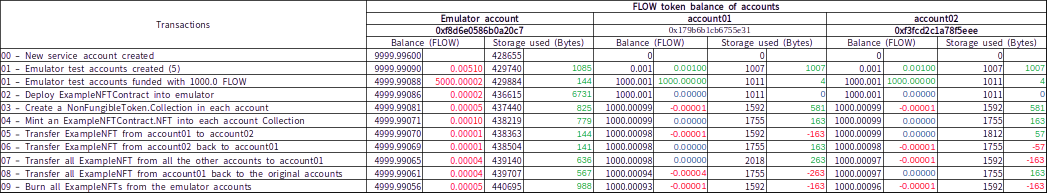
\includegraphics[width=1.0\textwidth]{../Images/09_FlowFeeCalculations.png}
    \caption{Fee and storage consumption in Flow}
    \label{fig:cadence_gas_cost}
\end{figure}

The main conclusion from analysing Table \ref{fig:cadence_gas_cost} is that the majority of transactions are priced to the minimum value of 0.000001 FLOW. This particular exercise included a service or emulator account and five additional user accounts. One interesting aspect to note is that the emulator account has costs with all operations, even when the account is not included in the transaction. This is because NFT operations, such as transfers, are run from the implementing contract. Since it was the emulator account that deployed the main contract, anytime someone invokes an NFT function, the contract executions are paid by the deployer. Individual users, emulated as additional account, also incur in costs when they sign the transactions, as expected. But overall, it appears that in this simple example, the total transactions costs never exceeded the minimum value, and as such, the majority of the transactions were charged as that. In cases where it seems that a higher fee was paid, such as the 0.000005 FLOW paid by the emulator account during the final burn operation, this is actually 5 minimum transaction fees, one per each time the burn function was executed in the main contract. Given how much more cheap FLOW is compared to ETH, and how, apparently, for simple NFT interactions only the minimum fee gets charges, Flow appears to be a much more attractive economically then Ethereum.

\end{document}